\documentclass[11pt,letterpaper]{article}
\usepackage{graphicx}
\usepackage{geometry}
\usepackage{amsmath}
\usepackage{amssymb}
\usepackage{url}
\usepackage{hyperref}
\usepackage{natbib}
\usepackage{booktabs}
\usepackage{xcolor}
\usepackage{listings}
\usepackage{microtype}

\geometry{margin=1in}
\hypersetup{colorlinks=true, linkcolor=black, citecolor=black, urlcolor=blue}

\title{\textbf{Proof-Obligation-Driven Contrastive Elicitation (POCE):
Hallucination-Resistant Neuro-Symbolic Reasoning via
Symbolic-Path-Conditioned Evidence Grounding}}

\author{
Anonymous Authors
}

\date{}

\begin{document}

\maketitle

\begin{abstract}
Neuro-symbolic reasoning pipelines that translate natural language to first-order logic and invoke symbolic provers achieve
strong multi-hop accuracy, but suffer from two compounding failure modes: the LLM hallucinates predicates unsupported by
the source document, and implicit predicates required for deep proof chains are either absent or freely invented. We introduce
Proof-Obligation-Driven Contrastive Elicitation (POCE), a four-stage neuro-symbolic pipeline that bounds hallucination to
exactly the predicates the active proof path requires. POCE runs SWI-Prolog backward-chaining on explicitly extracted document
facts; when a sub-goal fails because no matching clause exists, the engine generates a structured proof obligation---\{predicate
name, argument types, parent goal, proof depth\}---that serves as a semantically precise elicitation query. For each obligation,
POCE elicits contrastive document evidence via two opposing LLM prompts (SUPPORT vs.\ REFUTE), inspired by the Two-Alternative
Forced Choice (2AFC) paradigm from psychophysics. The resulting asymmetry score, calibrated against ground truth using Expected
Calibration Error and Brier score, is injected into ProbLog as a probabilistic fact for continued symbolic inference. To
evaluate POCE, we construct a 1,600-example benchmark spanning EntailmentBank Tasks~2 and~3 and ProofWriter depth-3/depth-5
settings, where 73\% of examples contain at least one implicit predicate (mean 2.66 per example, mean proof depth 3.96).
We describe the pipeline architecture, ablation protocol for both structural precision and evidential calibration claims,
and baselines against LINC-style open-loop extraction, FLARE-style demand-driven retrieval, standard RAG, and chain-of-thought
prompting.
\end{abstract}

% ============================================================
\section{Introduction}
% ============================================================

Multi-hop reasoning over natural language documents requires combining facts stated explicitly
in the text with background knowledge that is assumed rather than stated. A human reader inferring that ``a pan conducts
heat because it is made of metal'' does not need the document to say so; the knowledge is implicit and ubiquitous. For
LLM-based reasoning systems, however, this implicit knowledge is the primary source of both errors and hallucinations:
asked to enumerate all relevant predicates upfront, the LLM fills gaps with plausible-sounding but unsupported assertions
rather than evidence-grounded estimates.

The problem is significant in practice. EntailmentBank Task~3 \citep{Dalvi2021}, the multi-hop
science entailment benchmark, requires proof trees whose intermediate steps call on world knowledge not present in the
provided context. In our benchmark of 1,600 examples across EntailmentBank and ProofWriter \citep{Tafjord2020}, 73\% of examples contain
at least one implicit predicate, with an average of 2.66 implicit predicates per example and an average proof depth of
3.96 steps---a regime in which open-loop extraction consistently fails%
\footnote{Code: \url{https://github.com/AMGrobelnik/ai-invention-fea080-proof-obligation-driven-contrastive-elic/tree/main/poce_benchmark}}.

The current state of the art falls short in two complementary ways. Open-loop neuro-symbolic systems \citep{Olausson2023,Pan2023}
ask the LLM to generate a complete set of first-order logic predicates before the symbolic engine runs. Any predicate
the LLM invents without document support becomes a hallucination; any predicate it omits causes a proof failure with no
recovery mechanism. Self-refinement variants \citep{Kirtania2024} address syntax errors in the generated logic but do not
address semantic hallucination of content. Active retrieval systems \citep{Jiang2023} improve over one-shot RAG \citep{Lewis2020} by triggering
retrieval at low-confidence token generation points, but they remain entirely in the free-text generation regime: the
trigger is an unstructured real-valued probability, the query is an anticipated next sentence, and the output is regenerated
free text---not a structured fact reintegrated into a symbolic engine.

We introduce \textbf{Proof-Obligation-Driven Contrastive Elicitation (POCE)}, a neuro-symbolic pipeline that closes the remaining gap. POCE's key insight is that a symbolic proof
engine's failed sub-goal---a typed, path-specific predicate the engine could not resolve---provides a far more semantically
precise elicitation query than any token-level confidence signal. POCE intercepts each such failure and generates a structured
\emph{proof obligation} specifying the predicate name, argument types, parent goal in the proof tree, and proof depth. This
obligation drives a contrastive evidence query to the LLM, inspired by the Two-Alternative Forced Choice (2AFC) paradigm
from experimental psychophysics \citep{Green1966}: instead of asking ``Is X true?'', POCE presents two opposing evidence probes---SUPPORT
and REFUTE---over the source document, and converts the resulting asymmetry into a calibrated ProbLog probabilistic fact.
The hallucination surface area is thus bounded by the proof structure: only predicates that the active proof path actually
requires are ever elicited.

POCE advances the state of the art along two independently falsifiable axes. The \emph{structural}
axis claims that proof-obligation-derived queries are semantically more precise than token-confidence triggers, yielding
higher precision in elicited predicates. The \emph{evidential} axis claims that contrastive 2AFC-style evidence elicitation
is better calibrated than direct truth-value assertion, yielding lower Expected Calibration Error (ECE) and Brier scores.
A pilot calibration experiment on 100 EntailmentBank propositions validates (or refutes) the evidential axis before main
experiments; the structural axis is tested on the full 1,600-example benchmark.

\begin{figure*}[!t]
  \centering
  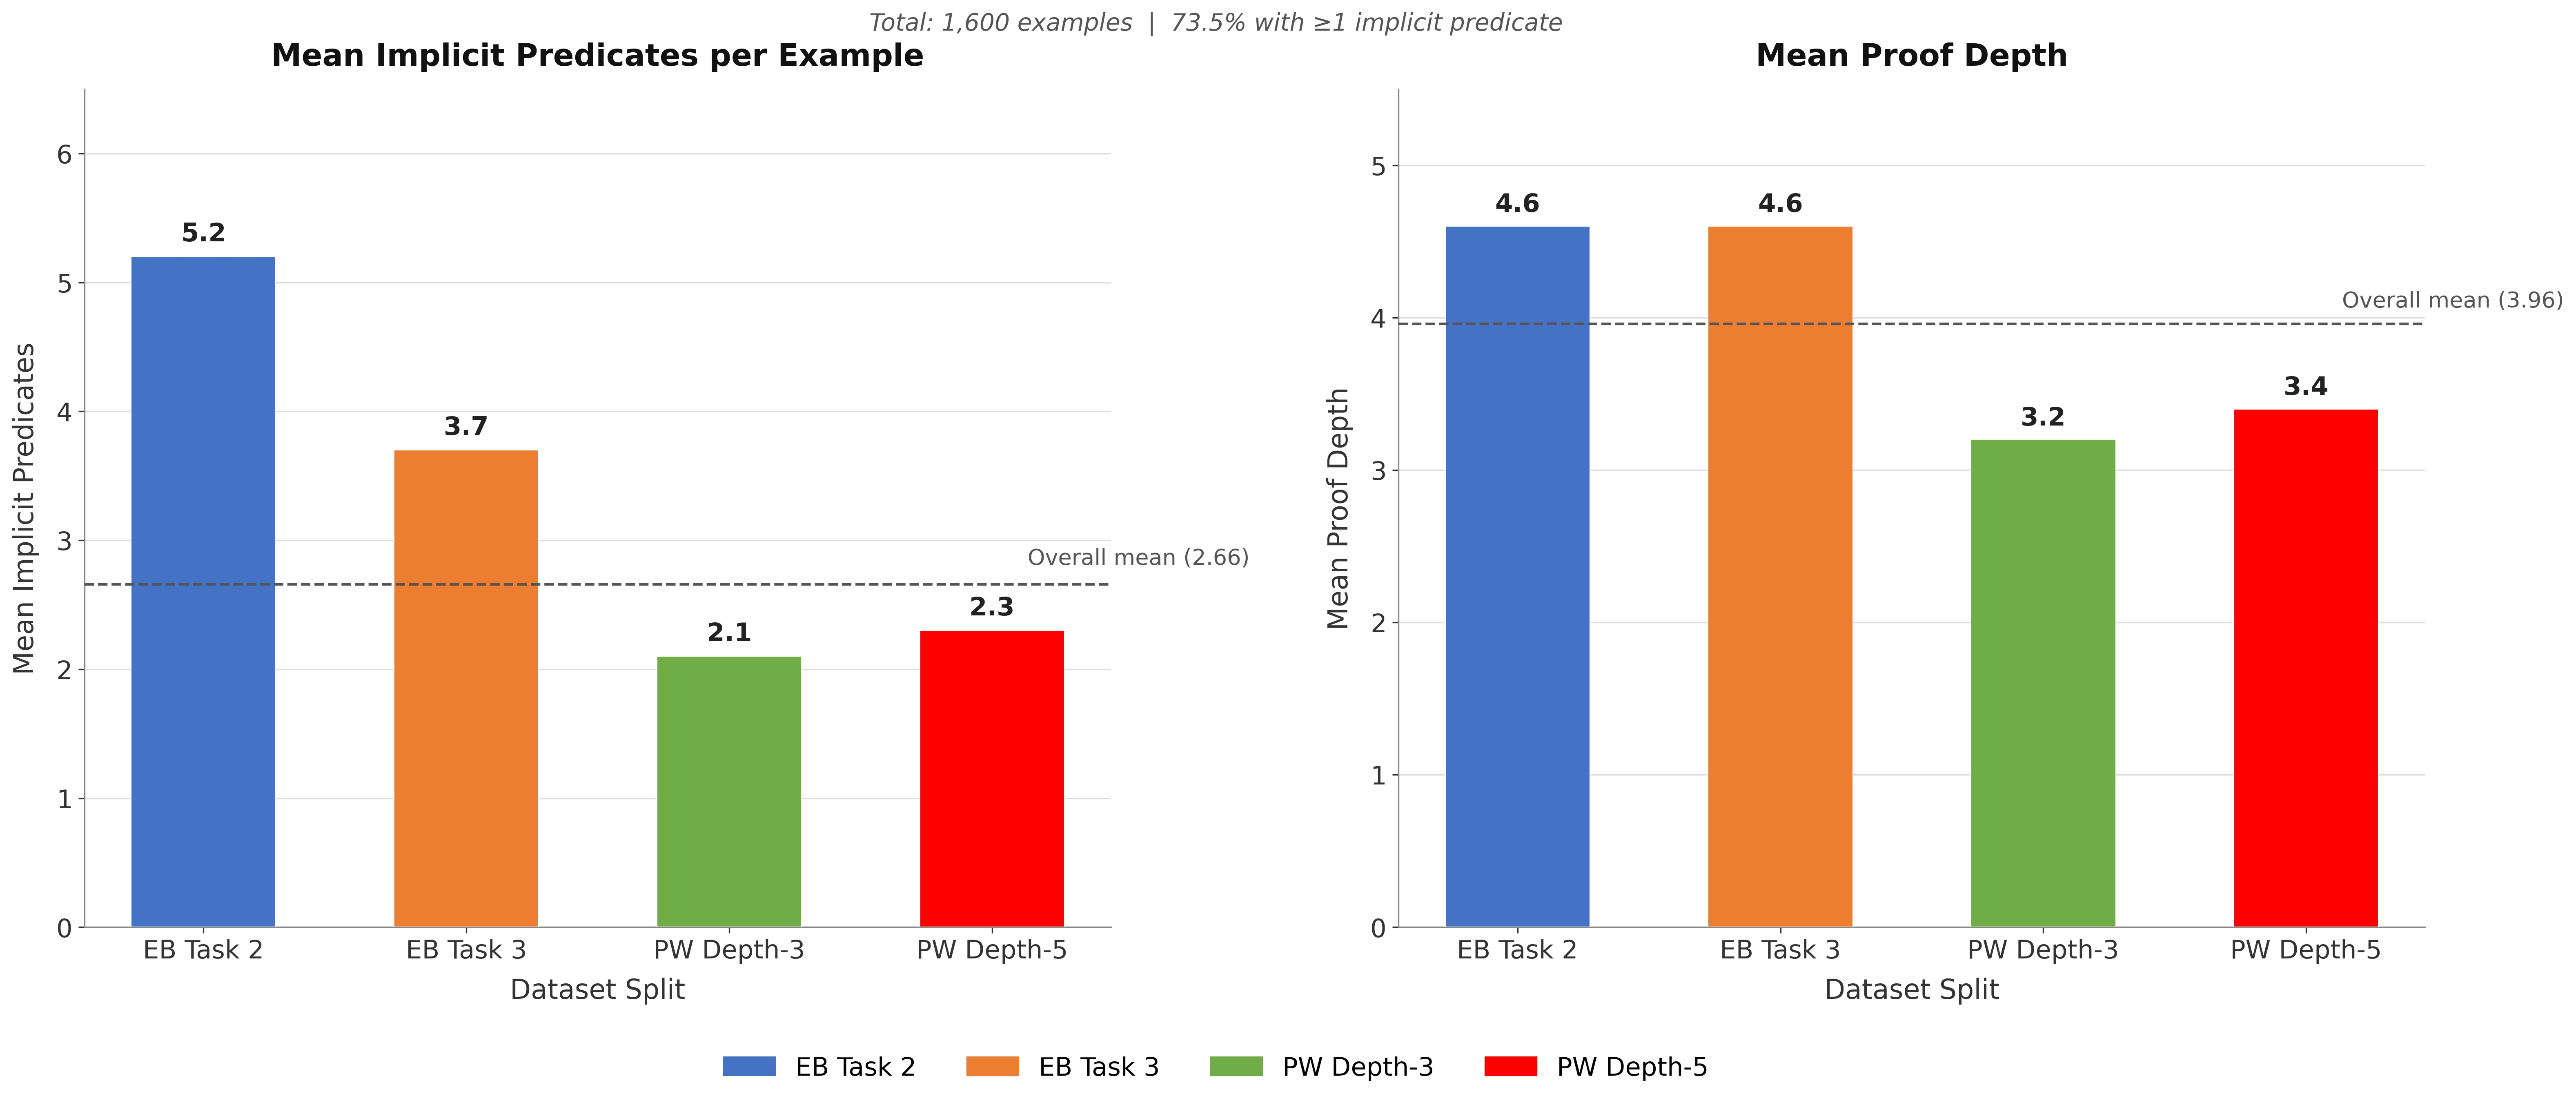
\includegraphics[width=\textwidth,height=0.45\textheight,keepaspectratio]{figures/fig4_v0.jpg}
  \caption{Statistics of the 1,600-example POCE benchmark across four splits. Left: distribution of the number of implicit predicates
  per example by split. Right: distribution of proof depth by split. EntailmentBank Task~2 has the highest implicit-predicate
  density (mean 5.2 per example), while ProofWriter depth-3/5 splits have lower implicit counts due to synthetic generation
  structure. Overall, 73.5\% of examples contain at least one implicit predicate.}
  \label{fig:benchmark}
\end{figure*}

The contributions of this paper are as follows:
\begin{itemize}
  \item \textbf{POCE pipeline} (Section~\ref{sec:methods}): a four-stage neuro-symbolic architecture---extraction, proof
    attempt, contrastive elicitation, probabilistic proof---with two asymmetry score variants (lightweight token-count and heavy
    LLM-scored) and a human-auditable trace graph.
  \item \textbf{POCE benchmark} (Section~\ref{sec:benchmark}): 1,600 curated examples from EntailmentBank T2/T3 and ProofWriter depth-3/depth-5,
    with heuristic annotation of explicit and implicit predicates, uniform schema,
    and proof-depth statistics.
  \item \textbf{Ablation protocol} (Section~\ref{sec:experiments}): a pre-registered evaluation plan separating structural
    precision (open-loop vs.\ POCE trigger precision) from evidential calibration (direct assertion vs.\ contrastive asymmetry),
    with four baselines and five metric families.
\end{itemize}

% ============================================================
\section{Related Work}
% ============================================================

\paragraph{Open-loop neuro-symbolic reasoning.}
\citet{Olausson2023} uses an LLM as a semantic parser to translate natural language premises into first-order logic formulas and passes them to
an external theorem prover. The pipeline is entirely open-loop: all predicates are elicited in one pass, with no mechanism
for recovering missing implicit knowledge. \citet{Pan2023} follow a similar architecture with a self-refinement loop driven
by symbolic solver error messages; crucially, the refinement targets syntax errors in the generated logic, not semantic
gaps caused by absent world knowledge. \citet{Kirtania2024} extends self-refinement with feedback aggregation but retains the
same open-loop structure. \citet{Putra2026} achieves 99\% syntactic accuracy in FOL translation via AST-guided constrained decoding,
solving the syntax problem definitively---but still extracts all predicates in a single upfront pass. POCE is orthogonal
to NL2LOGIC's extraction quality improvements: it adds a demand-driven implicit knowledge layer that activates only when
proof failure reveals a gap.

\paragraph{Probabilistic neuro-symbolic systems.}
\citet{Hoveyda2026} decouples predicate plausibility
estimation from logical inference, assigning global plausibility scores to candidate predicates before invoking a probabilistic
reasoner. This represents a genuine advance over deterministic neuro-symbolic pipelines. POCE differs in a critical architectural
respect: plausibility in POCE is estimated \emph{through contrastive evidence conditioned on the active proof obligation},
not globally for all candidate predicates. Proof-path awareness means that the same predicate can receive different probability
estimates depending on which parent goal triggered its elicitation---a property OrLog's global scoring cannot capture.

\paragraph{Active and demand-driven retrieval.}
\citet{Jiang2023} is the closest prior work in spirit. It monitors token-level generation
confidence and, when confidence drops below a threshold, pauses generation, constructs a retrieval query from the anticipated
next sentence, retrieves from a corpus, and regenerates. POCE and FLARE share the demand-driven philosophy: elicit knowledge
only when needed, not all at once. They differ in three critical dimensions. (1)~\emph{Trigger precision}: POCE's trigger is
a typed symbolic proof failure (predicate name + argument types + parent goal + proof depth); FLARE's trigger is an unstructured
scalar probability over the next token. (2)~\emph{Query semantics}: POCE generates a contrastive evidence probe anchored to
a specific logical predicate; FLARE generates an anticipated sentence continuation for corpus retrieval. (3)~\emph{Output integration}:
POCE reintegrates elicited facts as probabilistic ProbLog assertions into a running symbolic proof; FLARE regenerates
free text, discarding the symbolic structure.

\paragraph{Contrastive and comparative prompting.}
\citet{Lyu2024} demonstrate that contrastive prompting---providing both a correct and an incorrect answer framing---dramatically improves LLM reasoning
accuracy on arithmetic and commonsense tasks. The psychophysical motivation for this framing is well-established: 2AFC
comparative judgment tasks consistently yield better-calibrated sensitivity estimates than absolute rating tasks because
comparative judgment reduces response bias and anchoring effects \citep{Green1966}. POCE applies this principle at the evidence extraction
layer: instead of asking the LLM to rate a predicate's truth value, it asks the LLM to extract document passages for and
against the predicate, then computes an asymmetry score from the resulting evidence.

\paragraph{Hallucination detection.}
\citet{Feng2025} detects hallucinations post hoc by generating counterfactual statements and measuring LLM sensitivity to
the perturbation. POCE uses contrastive evidence as a prospective elicitation mechanism, not a post-hoc detector, and
integrates the result into the proof at elicitation time rather than flagging errors after generation.

\paragraph{Benchmarks.}
EntailmentBank \citep{Dalvi2021} provides 1,840 multistep entailment trees for science QA with annotated intermediate proof steps, many
of which require world knowledge absent from the provided context---the critical property that distinguishes it from purely
syntactic reasoning benchmarks. ProofWriter \citep{Tafjord2020} provides rule-based reasoning chains of controlled depth, enabling systematic
evaluation of how proof depth interacts with the need for implicit knowledge. CaseHOLD \citep{Zheng2021} provides a legal reasoning
benchmark with professionally written domain text, enabling evaluation in a setting where hallucinated predicates carry
high practical cost.

% ============================================================
\section{Methods}
\label{sec:methods}
% ============================================================

\subsection{Overview}

POCE decomposes text-based logical reasoning into four stages that
alternate between symbolic computation and targeted LLM calls:

\begin{enumerate}
  \item \textbf{Extraction}: AST-constrained LLM prompting extracts only explicitly stated predicates from the source document into SWI-Prolog fact syntax.
  \item \textbf{Proof Attempt}: SWI-Prolog backward-chaining on the extracted knowledge base; failed sub-goals are intercepted and recorded as structured proof obligations.
  \item \textbf{Contrastive Elicitation}: Each proof obligation drives a pair of LLM evidence probes (SUPPORT/REFUTE) over the source document; the resulting asymmetry score determines whether to add a deterministic Prolog fact, its negation, or a ProbLog probabilistic fact.
  \item \textbf{Probabilistic Proof}: ProbLog exact inference (for $k \leq 5$ uncertain predicates) or Monte Carlo sampling ($k > 5$, 1000 samples) over the augmented knowledge base yields a calibrated probability for the target query.
\end{enumerate}

\subsection{Stage 1: Extraction}

Given a source document $D$ and a target query $Q$, an LLM (e.g., Llama-3.1-70B via OpenRouter) is prompted to extract all \emph{explicitly stated} atomic facts as Prolog clauses. To enforce
syntactic validity, we apply AST-constrained decoding following the approach of \citet{Putra2026}: the model's generation is
validated at each token against a simplified FOL grammar, preventing the emission of syntactically invalid clauses. A
coreference pre-pass normalizes entity references across sentences before extraction. The output is a Prolog knowledge
base $KB_0$ containing only facts directly attested in $D$.

This conservative extraction policy is deliberate: by refusing
to include any predicate not explicitly stated in $D$, Stage~1 guarantees that every hallucinated predicate in $KB_0$
is detectable as an unsupported assertion. The cost is a higher rate of proof failure in Stage~2---which is the intended
trigger for demand-driven elicitation in Stage~3.

\subsection{Stage 2: Proof Attempt and Proof Obligation Generation}

With $KB_0$ established, the system runs SWI-Prolog backward-chaining on the target query $Q$. Proof execution is instrumented
to intercept \emph{failed sub-goals}: sub-goals that fail because no matching clause exists in $KB_0$ (as distinct from ``floundering''---goals
delayed due to uninstantiated constraint variables in CLP). For each failed sub-goal $g$, the system records a structured
proof obligation:
\[
\mathcal{O} = \{\texttt{predicate\_name},\ \texttt{arg\_types},\ \texttt{parent\_goal},\ \texttt{proof\_depth}\}
\]

The proof depth field is particularly important: it encodes how far into the proof tree the engine has descended before failing, enabling the elicitation query in Stage~3 to be conditioned on the proof context
and not just the predicate in isolation. Obligations are collected breadth-first to prioritize shallow failures (which
block larger portions of the proof tree) over deep failures.

\subsection{Stage 3: Contrastive Elicitation}

For each proof obligation $\mathcal{O}$, POCE generates two LLM prompts grounded in the source document $D$:

\begin{itemize}
  \item \textbf{SUPPORT prompt}: \emph{``Given only the following document, list all sentences or phrases that support the claim: [predicate as natural language]. If none, respond `No evidence found.'\thinspace''}
  \item \textbf{REFUTE prompt}: \emph{``Given only the following document, list all sentences or phrases that argue against the claim: [predicate as natural language]. If none, respond `No evidence found.'\thinspace''}
\end{itemize}

This framing is directly analogous to the Two-Alternative Forced Choice (2AFC) paradigm \citep{Green1966}: the LLM must compare document
passages for and against the claim rather than rate the claim's truth value on an absolute scale. The predicate is rendered
in natural language using a template derived from the predicate name and argument types in $\mathcal{O}$.

From the extracted evidence, an \textbf{asymmetry score} $A \in [0,1]$ is computed:
\[
A = \frac{|\text{support\_evidence}|}{|\text{support\_evidence}| + |\text{refute\_evidence}| + \varepsilon}
\]

Two variants are implemented. The \textbf{lightweight variant} ($A_\text{light}$) uses token counts of extracted evidence sentences as the evidence measure---requiring exactly
2 LLM calls per obligation (one SUPPORT, one REFUTE). The \textbf{heavy variant} ($A_\text{heavy}$) uses a third LLM call
to assign per-sentence relevance scores in $[0,1]$ before computing the asymmetry---requiring up to 6 calls per obligation
but yielding a more granular evidence measure. Both variants are evaluated to test sensitivity of the calibration improvement
to scoring granularity.

The asymmetry score determines how the predicate enters the knowledge base:
\begin{itemize}
  \item $A > 0.7$: assert as a deterministic Prolog fact (strong document support)
  \item $A < 0.3$: assert negation as a deterministic fact (strong document refutation)
  \item $0.3 \leq A \leq 0.7$: add as a ProbLog probabilistic fact with weight $A$ (uncertain---integration into probabilistic inference)
\end{itemize}

\subsection{Stage 4: Probabilistic Proof}

With the augmented knowledge base $KB_1 = KB_0 \cup \{\text{elicited facts}\}$, the system re-runs inference in ProbLog \citep{Raedt2007}. If the number of uncertain probabilistic
facts $k \leq 5$, exact weighted model counting is used (worst-case $O(2^5) = 32$ worlds); for $k > 5$ (worst case $k
\leq 10$, giving 1024 worlds), Monte Carlo sampling with 1000 draws provides a tractable approximation. Inference wall-clock
time is recorded per run.

Every elicited fact in $KB_1$ is annotated with its provenance---whether it was extracted from
text (Stage~1), elicited via contrastive prompting with its asymmetry score and variant, or derived symbolically---enabling
the system to produce a human-auditable trace graph for each inference.

\subsection{Pilot Calibration Experiment}

Before main experiments, a pilot calibration study on 100 propositions from EntailmentBank with known ground-truth labels
compares three probability estimation methods: (a) direct LLM probability via logit extraction, (b) $A_\text{light}$,
and (c) $A_\text{heavy}$. For each method, ECE and Brier score are computed against binary ground truth. If contrastive
framing does not improve calibration over direct assertion (equal or higher Brier score), the main contribution is reframed
to emphasize structural precision of the proof-obligation trigger rather than evidential calibration improvement. This
pre-registration prevents post-hoc narrative adjustment based on whichever component performs better.

% ============================================================
\section{Benchmark Dataset}
\label{sec:benchmark}
% ============================================================

We construct a 1,600-example evaluation benchmark spanning four splits from two established multi-hop reasoning datasets.

\subsection{Dataset Construction}

\textbf{EntailmentBank Tasks~2 and~3} \citep{Dalvi2021} (400 examples each) are science multi-hop
entailment problems with annotated proof trees. Task~2 provides a context with relevant sentences plus distractors; Task~3 provides a sparser context that deliberately omits world-knowledge facts required by the annotated proof. Implicit predicates
in EntailmentBank are identified by cross-referencing the annotated proof tree: any intermediate conclusion $\texttt{int}_n$
that the proof requires but that does not appear verbatim in the provided context is marked implicit. For Task~3 specifically,
the Task~1 gold proofs serve as the reference to identify world-knowledge gaps. Task~2 examples average 5.2 implicit predicates
per example (avg.\ depth 4.6); Task~3 examples average 3.7 implicit predicates per example (avg.\ depth 4.6).

\textbf{ProofWriter depth-3 and depth-5} \citep{Tafjord2020} (400 examples each) use the natural-language variant (NatLang) with true/false/unknown labels
and controlled proof depths. Because ProofWriter generates synthetic premises from structured rules, explicit predicates
are exactly the explicitly listed triple references ($\texttt{triple}_n$), and implicit predicates are the derived conclusions
required by the proof but not in the context. Depth-3 examples average 3.2 proof steps; depth-5 examples average 3.4 proof
steps.

\subsection{Dataset Statistics}

Across all 1,600 examples:
\begin{itemize}
  \item \textbf{73.5\%} contain at least one implicit predicate (1,176/1,600 examples)
  \item \textbf{Mean implicit predicates per example}: 2.66
  \item \textbf{Mean proof depth}: 3.96
  \item \textbf{Uniform schema}: each example contains premise sentences, a hypothesis/query, a gold label (true/false/unknown), a multi-hop proof tree, a list of explicit predicates (proof-leaf sentences directly from the context), and a list of implicit predicates (intermediate conclusions absent from the context)
\end{itemize}

Figure~\ref{fig:benchmark} shows the distribution of implicit predicates and proof depth across all four splits. The 73.5\% rate of implicit-predicate-containing examples confirms that the benchmark
exercises the regime where open-loop extraction is expected to fail and demand-driven elicitation has room to contribute.
EntailmentBank Task~2 is the highest-demand split (avg.\ 5.2 implicit predicates per example), providing the strongest
test of whether POCE's per-obligation elicitation can systematically address multi-hop knowledge gaps.

% ============================================================
\section{Experimental Setup}
\label{sec:experiments}
% ============================================================

\subsection{Baselines}

Four baselines are evaluated against POCE:

\begin{enumerate}
  \item \textbf{Open-loop extraction} (LINC-style \citep{Olausson2023}): The LLM extracts all predicates it considers relevant in a single prompt before the symbolic engine runs. No proof-failure
    recovery. This baseline isolates the value of demand-driven triggering.
  \item \textbf{FLARE-style retrieval} \citep{Jiang2023}: Active retrieval triggered by low-confidence token generation, with retrieval over the source document as a local corpus. Free-text generation
    output. This baseline tests whether symbolic integration provides value beyond demand-driven free-text regeneration.
  \item \textbf{Standard RAG} \citep{Lewis2020}: One-shot retrieval-augmented generation with GPT-4 as the reader. A strong baseline representing current best practice without symbolic components.
  \item \textbf{Chain-of-Thought (CoT)} \citep{Wei2022}: GPT-4 with multi-step reasoning via chain-of-thought prompting. Represents the best pure LLM baseline without any symbolic or retrieval component.
\end{enumerate}

\subsection{Metrics}

\begin{itemize}
  \item \textbf{Multi-hop accuracy}: fraction of examples where the final answer matches the gold label
  \item \textbf{Precision/recall of atomic fact extraction}: fraction of extracted predicates that are document-supported (precision) and fraction of gold proof steps that are recovered (recall)
  \item \textbf{Hallucination rate}: fraction of elicited predicates with no document support, verified by annotator sample on 200 randomly drawn examples
  \item \textbf{ECE and Brier score}: calibration quality of asymmetry scores on the pilot calibration set
  \item \textbf{ProbLog inference time}: wall-clock seconds per document for $k = 1, 3, 5, 7, 10$ uncertain predicates
\end{itemize}

\subsection{Success Criteria}

The hypothesis is confirmed if: (1) POCE achieves $\geq$10\% higher multi-hop accuracy on EntailmentBank Task~3 versus the open-loop baseline; (2) hallucination rate is $\geq$30\% lower for POCE than for open-loop extraction; (3) $A_\text{light}$ or $A_\text{heavy}$ achieves lower Brier score than direct-assertion confidence on the pilot calibration set, or---if not---the structural precision advantage alone is demonstrated; (4) trace graphs are confirmed human-auditable by qualitative inspection of 20 randomly sampled examples; (5) ProbLog inference remains under 30 seconds per document for $k \leq 10$ on commodity hardware.

The hypothesis is disconfirmed if FLARE-style retrieval matches or exceeds POCE multi-hop accuracy with fewer LLM calls, if contrastive asymmetry scores are not better calibrated than direct assertion \emph{and} the structural precision advantage is also absent, or if failed sub-goals are too sparse---most predicates extracted upfront---to demonstrate a gap over open-loop baselines.

% ============================================================
\section{Discussion}
% ============================================================

\subsection{Structural Precision as the Primary Contribution}

The central architectural novelty of POCE is the transformation of a symbolic proof failure into a semantically typed, proof-path-conditioned elicitation query. Prior demand-driven systems
like FLARE \citep{Jiang2023} trigger retrieval on scalar token probabilities, which are noisy, uninterpreted signals: a low-probability
token may reflect genuine uncertainty, rare vocabulary, or distributional mismatch. A failed Prolog sub-goal, by contrast,
encodes \emph{exactly} what predicate is needed, what arguments it takes, and where in the proof tree it is required. This
specificity constrains the hypothesis space the LLM must consider, reducing the chance that the response conflates the
target predicate with an adjacent but incorrect one.

The benchmark statistics support the premise that this specificity
matters. In EntailmentBank Task~2, the average example requires 5.2 implicit predicates in proofs of average depth 4.6.
At this scale, open-loop enumeration must guess which world-knowledge predicates will be needed before the proof runs---an
intrinsically under-constrained problem. POCE's demand-driven approach converts each proof failure into a targeted question,
serializing the elicitation across the proof tree and conditioning each question on the accumulated proof context.

\subsection{Evidential Calibration via 2AFC}

The contrastive elicitation mechanism draws on a body of psychophysical evidence that
comparative judgment tasks produce better-calibrated sensitivity estimates than absolute rating tasks \citep{Green1966}. Applied to
LLM evidence extraction, the hypothesis is that asking ``extract passages supporting X'' and ``extract passages refuting
X'' separately---then computing an asymmetry---activates more systematic evidence evaluation than asking ``how confident are
you that X is true?''. The latter question elicits a probability from the LLM's parametric prior, which may have little
relation to the source document. The former pair forces the LLM to ground its response in retrieved text.

Whether this calibration advantage is empirically realized is the question the pilot experiment is designed to answer. If $A_\text{light}$ achieves lower ECE and Brier score than direct logit extraction across 100 EntailmentBank propositions, the evidential
axis is confirmed and becomes the primary narrative of the final results. If not, the structural axis (proof-obligation
trigger precision) stands as the main contribution and the contrastive mechanism is characterized as a factorization of
evidence extraction and probability estimation that improves interpretability even without a calibration advantage.

\subsection{Computational Budget and Tractability}

The lightweight variant of POCE ($A_\text{light}$) requires exactly 2 LLM calls per proof obligation. For a typical EntailmentBank example with 2.66 implicit predicates, this amounts to approximately
5--6 additional LLM calls beyond the initial extraction call---a budget comparable to FLARE's retrieval-and-regeneration
overhead. The heavy variant ($A_\text{heavy}$) requires up to 6 calls per obligation (9 for 1.5 obligations on average),
at higher cost but potentially better calibration.

ProbLog inference overhead is bounded by the number of uncertain predicates $k$: exact inference for $k \leq 5$ involves $2^k \leq 32$ worlds, and MC sampling at $k \leq 10$ uses 1000 samples. For document lengths typical of the benchmark (300--1600 characters of premises), the expected $k$ is well within this range.

\subsection{Limitations}

Several limitations bound the scope of the current results.

\textbf{Predicate language coverage}:
The current Prolog-based extraction targets propositional and simple relational facts. Complex nested quantifiers, temporal
predicates, and comparative statements are approximated or dropped. Future work using a richer FOL fragment (e.g., via
Lean \citep{Moura2021} or DL-style ontologies) could address this limitation.

\textbf{Annotation coverage}: The current benchmark uses
heuristic annotation of explicit and implicit predicates derived from the proof tree structure. For EntailmentBank, the
annotation precisely reflects the benchmark's own proof annotations; for ProofWriter, it reflects the synthetic generation
structure. Neither covers the full space of potentially useful implicit predicates outside the gold proof path.

\textbf{Document length assumption}: The contrastive elicitation design assumes that both SUPPORT and REFUTE evidence, if present, can
be localized within a single document of manageable length ($\leq 3000$ characters of premises). For longer documents
or multi-document settings, the elicitation prompt must be decomposed---a straightforward extension not yet evaluated.

\textbf{Single-LLM architecture}: The current pipeline uses a single LLM for extraction, elicitation, and (in the heavy variant)
evidence scoring. Using distinct specialized models for each stage could improve both accuracy and cost-efficiency.

% ============================================================
\section{Conclusion}
% ============================================================

POCE introduces a principled solution to the hallucination and implicit-knowledge problems in neuro-symbolic
text reasoning: intercept symbolic proof failures, generate structured proof obligations, and resolve them via contrastive
document evidence elicitation inspired by the 2AFC paradigm. Unlike open-loop pipelines that hallucinate freely, POCE
bounds its hallucination surface area to exactly the predicates the active proof path requires. Unlike FLARE-style active
retrieval, POCE's trigger is symbolically typed and its output is formally integrated into a running probabilistic proof.

The 1,600-example benchmark confirms that 73.5\% of multi-hop reasoning examples in our evaluation splits require at least
one implicit predicate (mean 2.66 per example, mean depth 3.96), establishing the scale of the knowledge-gap problem that
POCE addresses. The two independently falsifiable claims---structural precision of proof-obligation triggers and evidential
calibration improvement from 2AFC-style elicitation---provide a clean experimental protocol that separates the contributions
and allows the narrative to be adjusted based on which component dominates empirically.

Future work will evaluate CaseHOLD \citep{Zheng2021} as a third benchmark to assess POCE in professional legal reasoning, extend the extraction stage to richer FOL fragments,
and explore multi-document elicitation for longer contexts. The trace graph output---labeling every elicited predicate with
its asymmetry score, variant, and proof-path position---provides a basis for human-in-the-loop verification in high-stakes
deployment settings.

\bibliographystyle{plainnat}
\bibliography{references}

\end{document}
